\documentclass[dvipdfmx]{beamer}

%
% Common preamble for all three parts.
%

\usepackage[english]{babel}
\usepackage{amsmath}
\usepackage{color}
\usepackage{minted}
\usepackage{hyperref}
\usepackage{multicol}
\usepackage{xcolor}
\usepackage{tabularx}
\usepackage{tikz}
\usetikzlibrary{arrows,intersections}
\usetikzlibrary{decorations.fractals}
\usepackage{tikz-cd}

\hypersetup{
    colorlinks=true,
    linkcolor=blue,
    filecolor=magenta,      
    urlcolor=cyan,
}
            
% Set Japanese font to Gothic
\usepackage[deluxe, expert]{otf}
\renewcommand{\kanjifamilydefault}{\gtdefault}

% Set math font
\usefonttheme{professionalfonts}
\newcommand{\im}{\mathrm{i}}

% only inline todonotes work
\usepackage{xkeyval}
\usepackage[textsize=small]{todonotes}
\presetkeys{todonotes}{inline}{}

\usetikzlibrary{shapes,arrows,positioning,shadows}

% no nav buttons
\usenavigationsymbolstemplate{}

\newcommand{\bftt}[1]{\textbf{\texttt{#1}}}
\newcommand{\comment}[1]{{\color[HTML]{008080}\textit{\textbf{\texttt{#1}}}}}
\newcommand{\cmd}[1]{{\color[HTML]{008000}\bftt{#1}}}
\newcommand{\bs}{\char`\\}
\newcommand{\cmdbs}[1]{\cmd{\bs#1}}
\newcommand{\lcb}{\char '173}
\newcommand{\rcb}{\char '175}
\newcommand{\cmdbegin}[1]{\cmdbs{begin\lcb}\bftt{#1}\cmd{\rcb}}
\newcommand{\cmdend}[1]{\cmdbs{end\lcb}\bftt{#1}\cmd{\rcb}}

\newcommand{\wllogo}{\textbf{Overleaf}}

% this is where the example source files are loaded from
% do not include a trailing slash
\newcommand{\fileuri}{https://raw.github.com/jdleesmiller/latex-course/master/en}

\newcommand{\wlserver}{https://www.overleaf.com}
\newcommand{\wlnewdoc}[1]{\wlserver/docs?snip\_uri=\fileuri/#1\&splash=none}

\def\tikzname{Ti\emph{k}Z}

% from http://tex.stackexchange.com/questions/5226/keyboard-font-for-latex
\newcommand*\keystroke[1]{%
  \tikz[baseline=(key.base)]
    \node[%
      draw,
      fill=white,
      drop shadow={shadow xshift=0.25ex,shadow yshift=-0.25ex,fill=black,opacity=0.75},
      rectangle,
      rounded corners=2pt,
      inner sep=1pt,
      line width=0.5pt,
      font=\scriptsize\sffamily
    ](key) {#1\strut}
  ;
}
\newcommand{\keystrokebftt}[1]{\keystroke{\bftt{#1}}}


\let\olditemize\itemize
\renewcommand{\itemize}{
\olditemize
\setlength{\itemsep}{1.2pt}
\setlength{\parskip}{5pt}
\setlength{\parsep}{10pt}
}


% stolen from minted.dtx
\newenvironment{exampletwoup}
  {\VerbatimEnvironment
   \begin{VerbatimOut}{example.out}}
  {\end{VerbatimOut}
   \setlength{\parindent}{0pt}
   \fbox{\begin{tabular}{l|l}
   \begin{minipage}{0.55\linewidth}
     \inputminted[fontsize=\small,resetmargins]{latex}{example.out}
   \end{minipage} &
   \begin{minipage}{0.35\linewidth}
     \input{example.out}
   \end{minipage}
   \end{tabular}}}

\newenvironment{exampletwouptiny}
  {\VerbatimEnvironment
   \begin{VerbatimOut}{example.out}}
  {\end{VerbatimOut}
   \setlength{\parindent}{0pt}
   \fbox{\begin{tabular}{l|l}
   \begin{minipage}{0.55\linewidth}
     \inputminted[fontsize=\scriptsize,resetmargins]{latex}{example.out}
   \end{minipage} &
   \begin{minipage}{0.35\linewidth}
     \setlength{\parskip}{6pt plus 1pt minus 1pt}%
     \raggedright\scriptsize\input{example.out}
   \end{minipage}
   \end{tabular}}}

\newenvironment{exampletwouptinynoframe}
  {\VerbatimEnvironment
   \begin{VerbatimOut}{example.out}}
  {\end{VerbatimOut}
   \setlength{\parindent}{0pt}
   \begin{tabular}{l|l}
   \begin{minipage}{0.55\linewidth}
     \inputminted[fontsize=\scriptsize,resetmargins]{latex}{example.out}
   \end{minipage} &
   \begin{minipage}{0.35\linewidth}
     \setlength{\parskip}{6pt plus 1pt minus 1pt}%
     \raggedright\scriptsize\input{example.out}
   \end{minipage}
   \end{tabular}}
   


\title{\LaTeX 講習会}
\author{森脇 可奈}
\date{2022年9月29日}
\medskip
\subtitle{物理学科内定者向けガイダンス}

\titlegraphic{%

\includegraphics[height=40pt]{UT_Science_logo.jpg}
}

\begin{document}

%%%%%%%%%%%%%%%%%%%%%%%%%%%%%%%%%%%%%%%%%%%%%%%%%%%%%%%%%%%%%%%%%%%%%%%%%%%%%%%
%%%%%%%%%%%%%%%%%%%%%%%%%%%%%%%%%%%%%%%%%%%%%%%%%%%%%%%%%%%%%%%%%%%%%%%%%%%%%%%
%%%%%%%%%%%%%%%%%%%%%%%%%%%%%%%%%%%%%%%%%%%%%%%%%%%%%%%%%%%%%%%%%%%%%%%%%%%%%%%
\begin{frame}
\titlepage
\centering
\footnotesize{講習会の HP \url{https://www.phys.s.u-tokyo.ac.jp/about/35200/} から\\「当日課題」をダウンロードしてください。パスワードは「\textcolor{magenta}{kadai2022}」です。}

\end{frame}

%%%%%%%%%%%%%%%%%%%%%%%%%%%%%%%%%%%%%%%%%%%%%%%%%%%%%%%%%%%%%%%%%%%%%%%%%%%%%%%
%%%%%%%%%%%%%%%%%%%%%%%%%%%%%%%%%%%%%%%%%%%%%%%%%%%%%%%%%%%%%%%%%%%%%%%%%%%%%%%
%%%%%%%%%%%%%%%%%%%%%%%%%%%%%%%%%%%%%%%%%%%%%%%%%%%%%%%%%%%%%%%%%%%%%%%%%%%%%%%
\begin{frame}{この講習会の内容}
\begin{itemize}
    \item Overleaf を用いて \LaTeX の基本的な使い方を学ぶ
    
    \bigskip
    \item \textcolor{teal}{目標}:当日課題の1ページ目を自分で再現する
    \begin{figure}
        \centering
        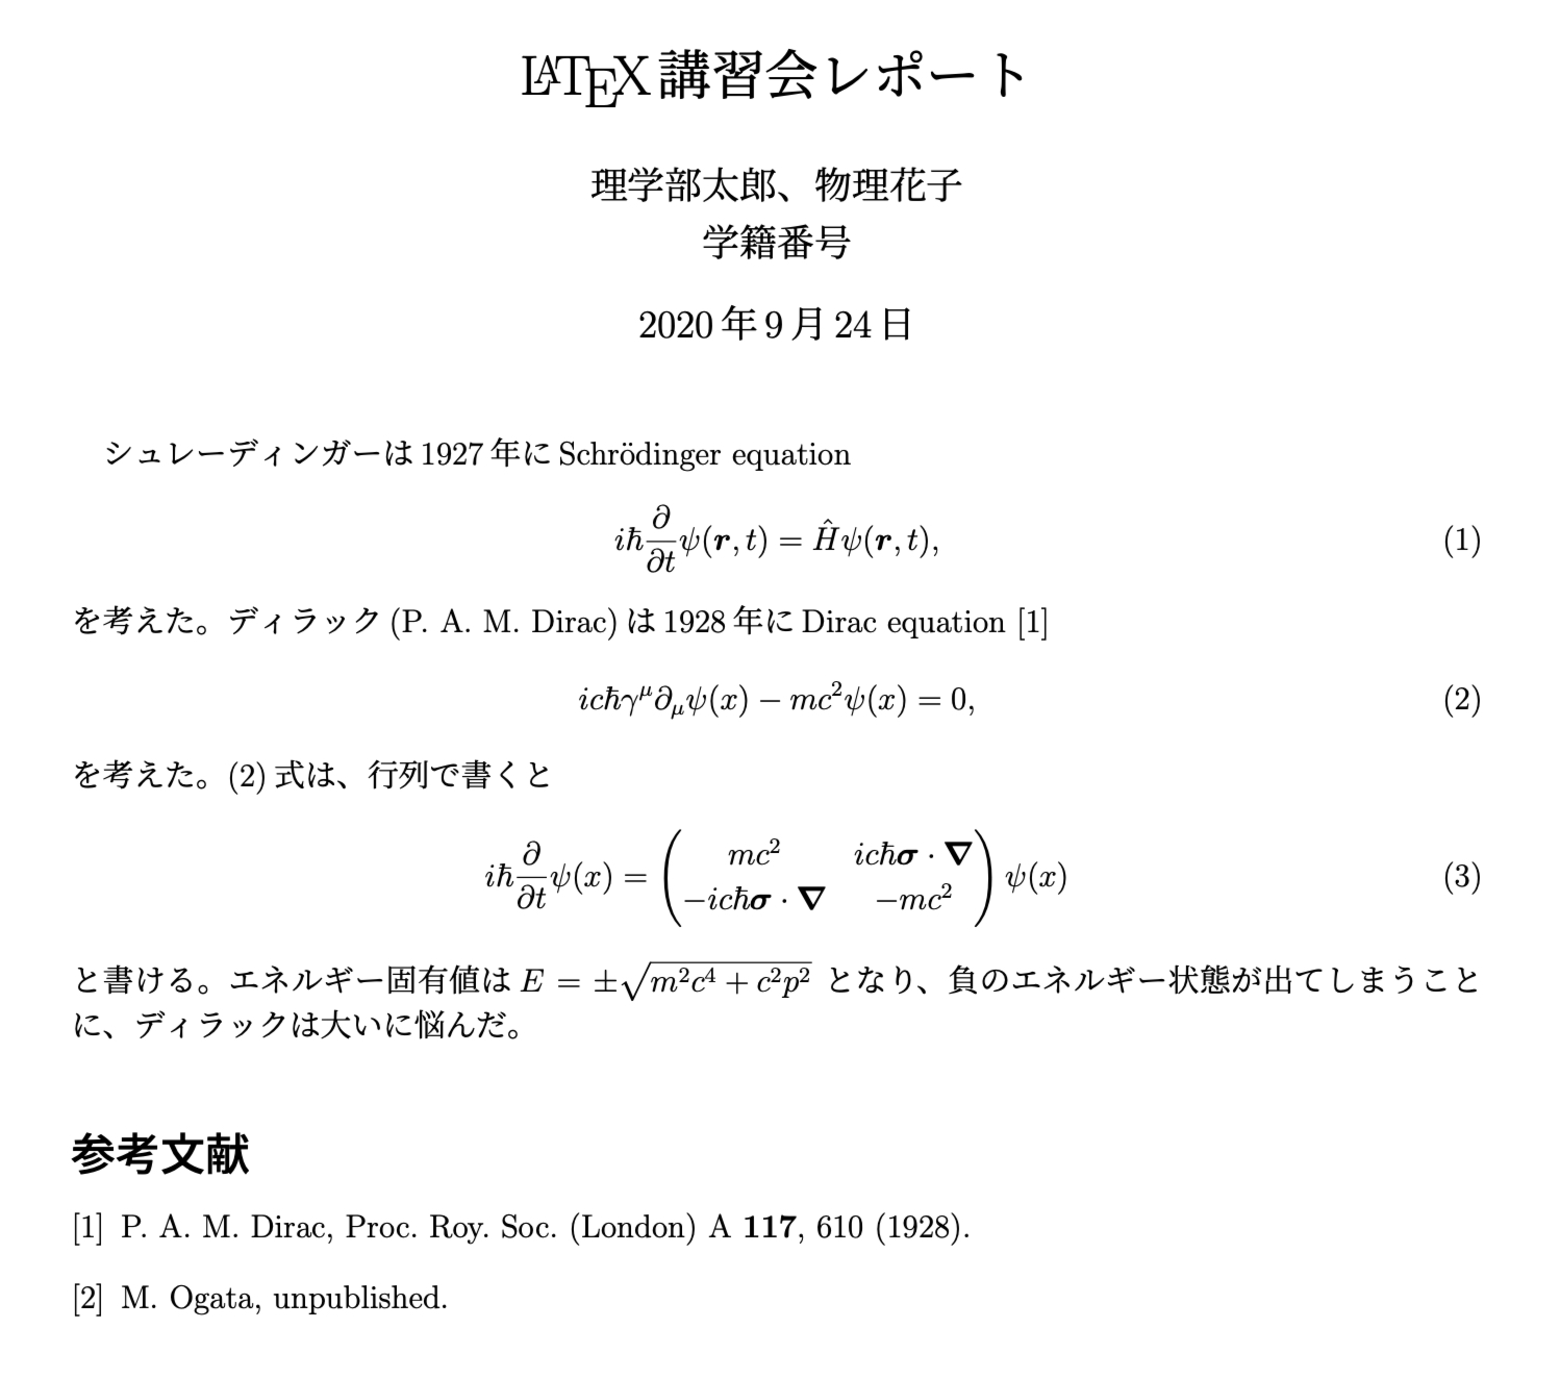
\includegraphics[width=8cm]{fig_kadai.pdf}
    \end{figure}
\end{itemize}
\end{frame}

%%%%%%%%%%%%%%%%%%%%%%%%%%%%%%%%%%%%%%%%%%%%%%%%%%%%%%%%%%%%%%%%%%%%%%%%%%%%%%%
%%%%%%%%%%%%%%%%%%%%%%%%%%%%%%%%%%%%%%%%%%%%%%%%%%%%%%%%%%%%%%%%%%%%%%%%%%%%%%%
%%%%%%%%%%%%%%%%%%%%%%%%%%%%%%%%%%%%%%%%%%%%%%%%%%%%%%%%%%%%%%%%%%%%%%%%%%%%%%%
\begin{frame}[fragile]{準備:新しい文書の作成}
\begin{itemize}
    \item Overleaf にログインする
    \item 「New Project」→「Blank Project」を選択し、適当な名前(例: LaTeX講習会)を入力して「Create」を押す
\end{itemize}
\begin{figure}
    \centering
    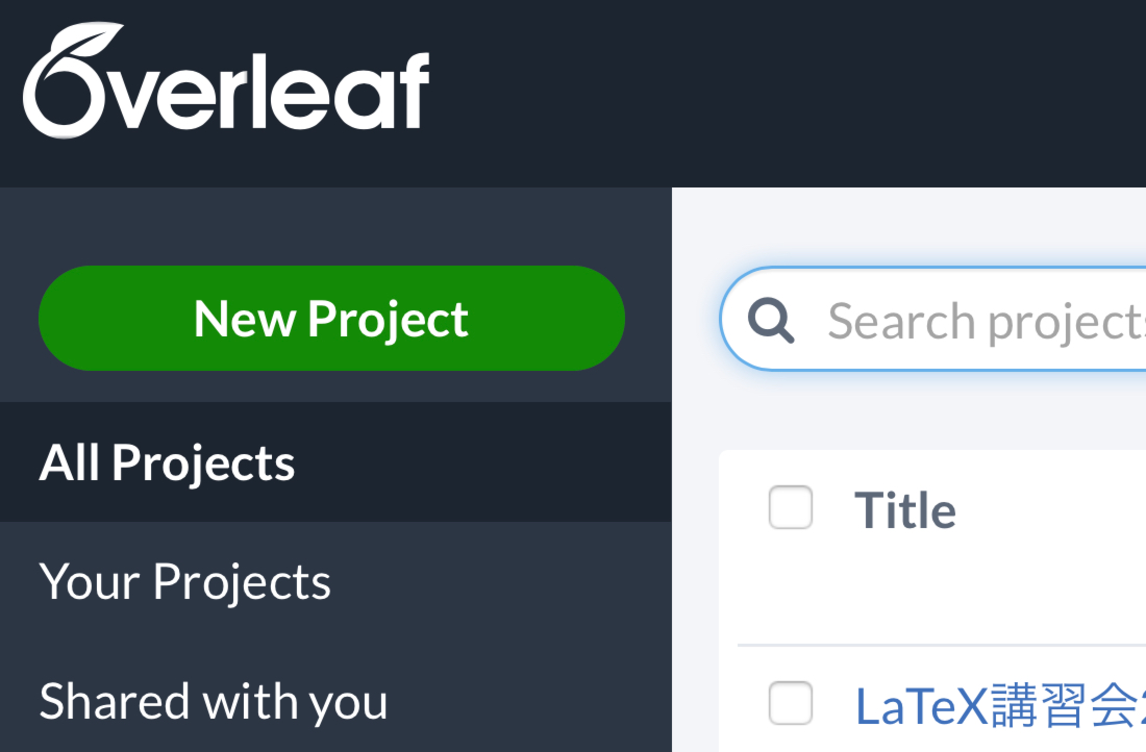
\includegraphics[width=7cm,pagebox=cropbox,clip]{NewDocument}
\end{figure}
\end{frame}

%%%%%%%%%%%%%%%%%%%%%%%%%%%%%%%%%%%%%%%%%%%%%%%%%%%%%%%%%%%%%%%%%%%%%%%%%%%%%%%
%%%%%%%%%%%%%%%%%%%%%%%%%%%%%%%%%%%%%%%%%%%%%%%%%%%%%%%%%%%%%%%%%%%%%%%%%%%%%%%
%%%%%%%%%%%%%%%%%%%%%%%%%%%%%%%%%%%%%%%%%%%%%%%%%%%%%%%%%%%%%%%%%%%%%%%%%%%%%%%
\begin{frame}[fragile]{準備:Overleaf での日本語環境の設定}
\begin{itemize}
    \item 左上のファイルアイコンをクリックして、「New File」を選択、「File Name」に「\textcolor{magenta}{latexmkrc}」を指定して「Create」を押す
    \begin{figure}
        \centering
        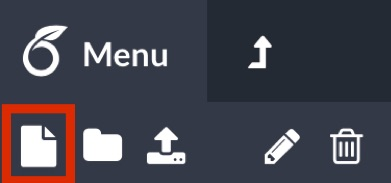
\includegraphics[height=1.5cm]{fig_new_file.jpg}
        \qquad
        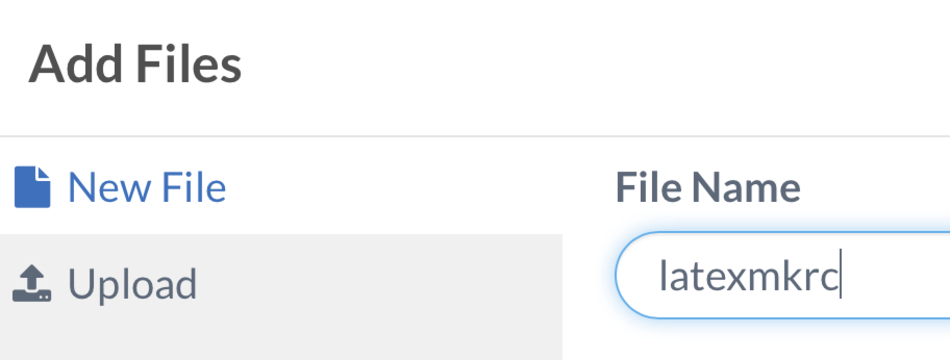
\includegraphics[height=1.5cm]{fig_latexmkrc.pdf}
    \end{figure}
    
    \item 左のファイル一覧に「latexmkrc」が現れるので選択し、以下の通り入力する
    \begin{minted}[frame=single]{bash}
    $latex      = 'uplatex';
    $bibtex     = 'uplatex';
    $dvipdf     = 'dvipdfmx %O -o %D %S';
    $makeindex  = 'mendex %O -o %D %S';
    $pdf_mode   = 3;
    \end{minted}
\end{itemize}
\alert{注}:「latexmkrc」と「main.tex」は同じフォルダ内に置く
\end{frame}

%%%%%%%%%%%%%%%%%%%%%%%%%%%%%%%%%%%%%%%%%%%%%%%%%%%%%%%%%%%%%%%%%%%%%%%%%%%%%%%
%%%%%%%%%%%%%%%%%%%%%%%%%%%%%%%%%%%%%%%%%%%%%%%%%%%%%%%%%%%%%%%%%%%%%%%%%%%%%%%
%%%%%%%%%%%%%%%%%%%%%%%%%%%%%%%%%%%%%%%%%%%%%%%%%%%%%%%%%%%%%%%%%%%%%%%%%%%%%%%
\begin{frame}{準備:Overleaf での日本語環境の設定(続き)}
\begin{itemize}
    \item 左上の「Menu」ボタンを押して、「Compiler」に「LaTeX」を選択する
    \begin{figure}
        \centering
        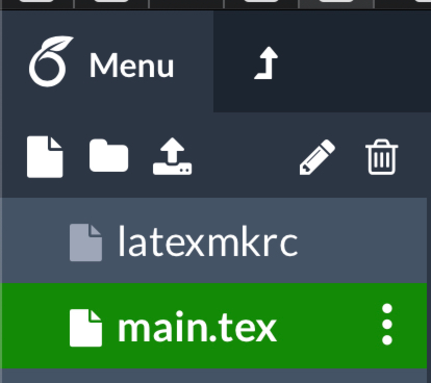
\includegraphics[height=3cm]{Menu.pdf}\qquad
        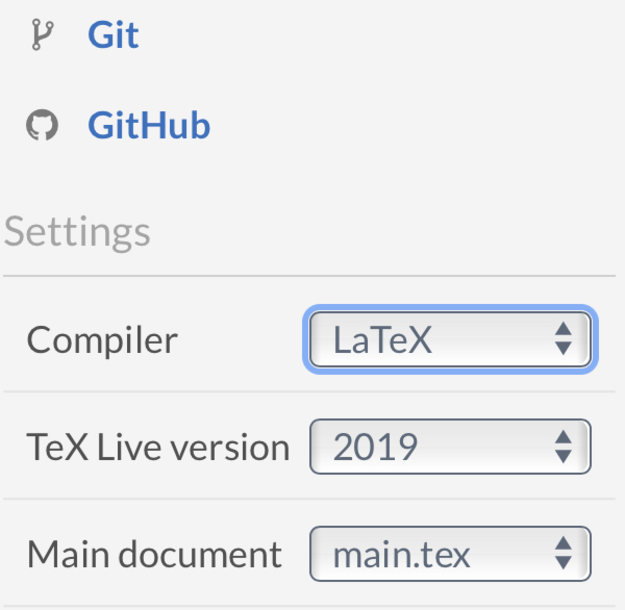
\includegraphics[height=3cm]{Compiler.pdf}
    \end{figure}
    \item 「main.tex」をクリックし「Recompile」ボタンを押すと、PDFファイルが作成される
    \begin{figure}
        \centering
        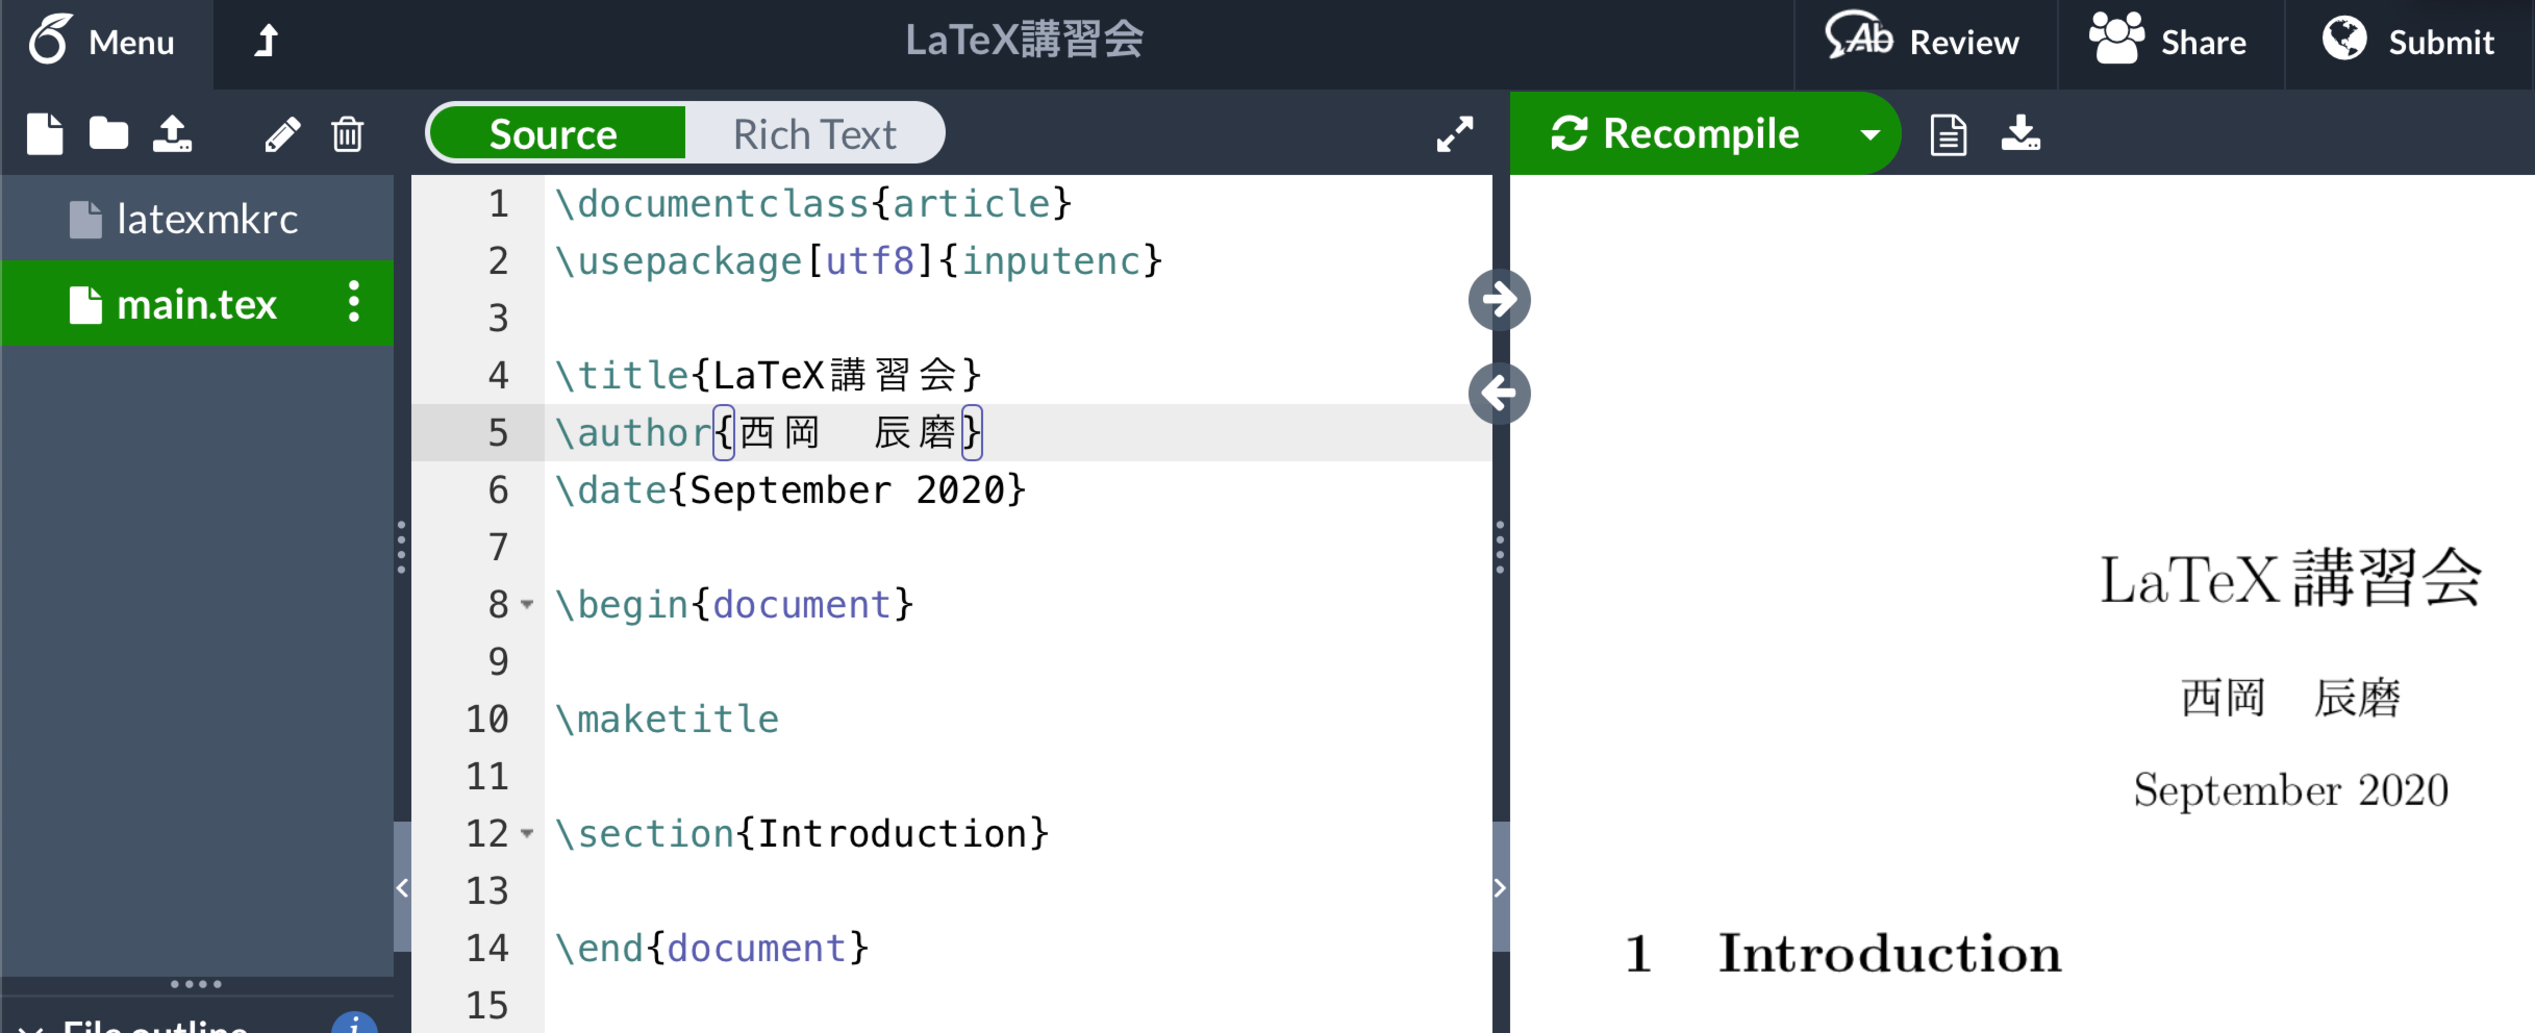
\includegraphics[height=3cm]{fig_preview.pdf}
    \end{figure}
\end{itemize}
\end{frame}

%%%%%%%%%%%%%%%%%%%%%%%%%%%%%%%%%%%%%%%%%%%%%%%%%%%%%%%%%%%%%%%%%%%%%%%%%%%%%%%
%%%%%%%%%%%%%%%%%%%%%%%%%%%%%%%%%%%%%%%%%%%%%%%%%%%%%%%%%%%%%%%%%%%%%%%%%%%%%%%
%%%%%%%%%%%%%%%%%%%%%%%%%%%%%%%%%%%%%%%%%%%%%%%%%%%%%%%%%%%%%%%%%%%%%%%%%%%%%%%
\begin{frame}[fragile]{\LaTeX{} の特徴}
\begin{itemize}
\item \LaTeX は「ラテック」や「ラテフ」などと呼ばれる組版処理システム
%
\bigskip
\item 特に数式入りの文章が簡単に作成できる:
    \begin{itemize}
        \item $y=x^2 + 1$, $e^{\im\,\theta} = \cos\theta + \im\,\sin\theta$, $\zeta(s) = \sum_{n=1}^\infty\,n^{-s}$, $\cdots$
    \end{itemize}
%
\bigskip
\item 様々なパッケージがあり、どんな文章も作成できる:
    \begin{itemize}
    \item 論文やレポート、プレゼンテーション用スライド(\href{https://www.overleaf.com/learn/latex/Beamer}{Beamer})、描画(\href{https://www.overleaf.com/learn/latex/TikZ_package}{TikZ})、 \ldots
    \end{itemize}
\begin{center}
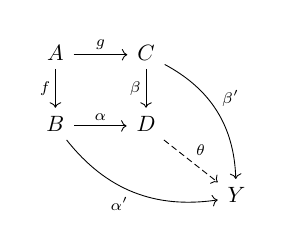
\begin{tikzpicture}[baseline= (a).base]
\node[scale=.8] (a) at (0,0){
\begin{tikzcd}
A \arrow[d,"f"'] \arrow[r,"g"] &
C \arrow[d,"\beta"'] \arrow[ddr,bend left,"\beta'"] \\
B \arrow[r,"\alpha"] \arrow[drr,bend right,"\alpha'"'] &
D \arrow[dr,dashed,"\theta"] \\
&& Y
\end{tikzcd}
};
\end{tikzpicture}
\qquad
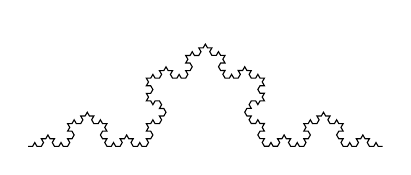
\begin{tikzpicture}[scale=1.5,decoration=Koch snowflake]
\draw decorate{ decorate{ decorate{ decorate{ (0,-1) -- (3,-1) }}}};
\end{tikzpicture}
\end{center}
\end{itemize}
\end{frame}

%%%%%%%%%%%%%%%%%%%%%%%%%%%%%%%%%%%%%%%%%%%%%%%%%%%%%%%%%%%%%%%%%%%%%%%%%%%%%%%
%%%%%%%%%%%%%%%%%%%%%%%%%%%%%%%%%%%%%%%%%%%%%%%%%%%%%%%%%%%%%%%%%%%%%%%%%%%%%%%
%%%%%%%%%%%%%%%%%%%%%%%%%%%%%%%%%%%%%%%%%%%%%%%%%%%%%%%%%%%%%%%%%%%%%%%%%%%%%%%
\begin{frame}[fragile]{\LaTeX の仕組み}
\begin{itemize}
\item 普通の文章と \LaTeX 特有の\cmd{コマンド}を使って文章を書く
\item \LaTeX でコンパイルすると組版された文章ができあがる
\end{itemize}
\vskip 2ex
\begin{center}
\begin{minted}[frame=single]{latex}
\LaTeX では $\backslash$ から始まる特殊なコマンドを使う
\end{minted}
\vskip 2ex
\tikz\node[single arrow,fill=gray!50,%font=\ttfamily\bfseries,%
  rotate=270,xshift=-1em]{\LaTeX};
\vskip 2ex
\fbox{\LaTeX では $\backslash$ から始まる特殊なコマンドを使う}
\end{center}
\end{frame}

%%%%%%%%%%%%%%%%%%%%%%%%%%%%%%%%%%%%%%%%%%%%%%%%%%%%%%%%%%%%%%%%%%%%%%%%%%%%%%%
%%%%%%%%%%%%%%%%%%%%%%%%%%%%%%%%%%%%%%%%%%%%%%%%%%%%%%%%%%%%%%%%%%%%%%%%%%%%%%%
%%%%%%%%%%%%%%%%%%%%%%%%%%%%%%%%%%%%%%%%%%%%%%%%%%%%%%%%%%%%%%%%%%%%%%%%%%%%%%%
\begin{frame}[fragile]{いくつかの例}
\begin{exampletwoup}
\begin{itemize}
    \item \textrm{Roman}
    \item \textit{Italic}
    \item \textbf{Bold}
\end{itemize}
\end{exampletwoup}
\vskip 2ex
\begin{exampletwoup}
\begin{figure}
    
\includegraphics[height=1cm]
    {UT_Science_logo.jpg}
\end{figure}
\end{exampletwoup}
\vskip 2ex
\begin{exampletwoup}
\begin{equation}
    \alpha + \beta + 1
\end{equation}
\end{exampletwoup}
\end{frame}

%%%%%%%%%%%%%%%%%%%%%%%%%%%%%%%%%%%%%%%%%%%%%%%%%%%%%%%%%%%%%%%%%%%%%%%%%%%%%%%
%%%%%%%%%%%%%%%%%%%%%%%%%%%%%%%%%%%%%%%%%%%%%%%%%%%%%%%%%%%%%%%%%%%%%%%%%%%%%%%
%%%%%%%%%%%%%%%%%%%%%%%%%%%%%%%%%%%%%%%%%%%%%%%%%%%%%%%%%%%%%%%%%%%%%%%%%%%%%%%
\begin{frame}[fragile]{簡単な \LaTeX{} の文章}
\begin{minted}[frame=single]{latex}
\documentclass[uplatex,dvipdfmx]{jsarticle}
\begin{document}
    吾輩は猫である名前はまだ無い
    %ここはコメントです
\end{document}
\end{minted}
\medskip
\begin{itemize}
\item コマンドは\textcolor{blue}{バックスラッシュ} \keystrokebftt{\bs}から始まる
\item 全ての文章は \cmdbs{documentclass} から始まる
\item カッコ \keystrokebftt{\{} \keystrokebftt{\}}の中の引数は文章の種類を表す\\
日本語の文章では \textcolor{magenta}{\bftt{jarticle}} もしくは \textcolor{magenta}{\bftt{jsarticle}} を使う
\item パーセント \keystrokebftt{\%}の後の文章はコメントで、 \LaTeX{} でコンパイル後は\textcolor{red}{表示されない}
\end{itemize}
\end{frame}

%%%%%%%%%%%%%%%%%%%%%%%%%%%%%%%%%%%%%%%%%%%%%%%%%%%%%%%%%%%%%%%%%%%%%%%%%%%%%%%
%%%%%%%%%%%%%%%%%%%%%%%%%%%%%%%%%%%%%%%%%%%%%%%%%%%%%%%%%%%%%%%%%%%%%%%%%%%%%%%
%%%%%%%%%%%%%%%%%%%%%%%%%%%%%%%%%%%%%%%%%%%%%%%%%%%%%%%%%%%%%%%%%%%%%%%%%%%%%%%
\begin{frame}[fragile]{タイプセットの基本}
\small
\begin{itemize}
\item 文章は \cmdbegin{document} と \cmdend{document} の間に書く
\item 普通の文章はそのまま表示される

\medskip
\begin{exampletwouptiny}
吾輩は猫である名前はまだ無い

どこで生れたかとんと見当がつかぬ
何でも薄暗いじめじめした所で
ニャーニャー泣いていた事だけは記憶している
吾輩はここで始めて人間というものを見た
\end{exampletwouptiny}
\item \textcolor{magenta}{2つ以上の半角の空白}は詰めて表示される(全角は詰めない)

\medskip
\begin{exampletwouptiny}
吾輩は  猫である      %半角2つの空白

吾輩は  猫である    %全角2つの空白
\end{exampletwouptiny}
\end{itemize}
\end{frame}

%%%%%%%%%%%%%%%%%%%%%%%%%%%%%%%%%%%%%%%%%%%%%%%%%%%%%%%%%%%%%%%%%%%%%%%%%%%%%%%
%%%%%%%%%%%%%%%%%%%%%%%%%%%%%%%%%%%%%%%%%%%%%%%%%%%%%%%%%%%%%%%%%%%%%%%%%%%%%%%
%%%%%%%%%%%%%%%%%%%%%%%%%%%%%%%%%%%%%%%%%%%%%%%%%%%%%%%%%%%%%%%%%%%%%%%%%%%%%%%
\begin{frame}[fragile]{タイプセットに関する注意点}
\small
\begin{itemize}
\item \LaTeX では次の特殊記号(エスケープ記号)は特別な役割を持つ:
\begin{center}
\begin{tabular}{cccccccccc}
\keystrokebftt{\{} &
\keystrokebftt{\}} &
\keystrokebftt{\%} &
\keystrokebftt{\#} &
\keystrokebftt{\&} &
\keystrokebftt{\$} & 
\keystrokebftt{\_} &
\keystrokebftt{\bs} &
\keystrokebftt{\textasciitilde} &
\keystrokebftt{\textasciicircum}
\end{tabular}
\end{center}
    \begin{itemize}
        \item \keystrokebftt{\%}:コメント
        \item \keystrokebftt{\&}:表などで文字の位置を揃える
        \item \keystrokebftt{\$}:数式モード
    \end{itemize}
\bigskip
\item これらの記号を表示するには次のようにすればよい:

\medskip
\begin{exampletwoup}
\{ \} \% \# \& \$ \_
\textbackslash
\textasciitilde
\textasciicircum
\end{exampletwoup}
\end{itemize}
\end{frame}

%%%%%%%%%%%%%%%%%%%%%%%%%%%%%%%%%%%%%%%%%%%%%%%%%%%%%%%%%%%%%%%%%%%%%%%%%%%%%%%
%%%%%%%%%%%%%%%%%%%%%%%%%%%%%%%%%%%%%%%%%%%%%%%%%%%%%%%%%%%%%%%%%%%%%%%%%%%%%%%
%%%%%%%%%%%%%%%%%%%%%%%%%%%%%%%%%%%%%%%%%%%%%%%%%%%%%%%%%%%%%%%%%%%%%%%%%%%%%%%
\begin{frame}[fragile]{数式の書き方: \keystrokebftt{\$} を使う方法}
\begin{itemize}
\item \keystrokebftt{\$} 記号で囲まれた文字は数式として\textcolor{teal}{文中}に表示される:

\medskip
\begin{exampletwouptiny}
% 数式ではない例:
a と b を異なる正の数とし、
c = a - b + 1 とおく

% 数式の例:
$a$ と $b$ を異なる正の数とし、
$c = a - b + 1$ とおく
\end{exampletwouptiny}

\bigskip
\item 注1:\keystrokebftt{\$} 記号は常にペアで用いて、間には\textcolor{magenta}{半角文字}を使う
\item 注2:\keystrokebftt{\$} の代わりに \textbackslash ( と \textbackslash ) で囲んでも良い
\item 注3:\LaTeX{} は\textcolor{blue}{数式中の半角空白を無視}する:

\medskip
\begin{exampletwouptiny}
$y=mx+b$ を変形して \ldots

$y = m x + b $ を変形して \ldots
\end{exampletwouptiny}
\end{itemize}
\end{frame}

%%%%%%%%%%%%%%%%%%%%%%%%%%%%%%%%%%%%%%%%%%%%%%%%%%%%%%%%%%%%%%%%%%%%%%%%%%%%%%%
%%%%%%%%%%%%%%%%%%%%%%%%%%%%%%%%%%%%%%%%%%%%%%%%%%%%%%%%%%%%%%%%%%%%%%%%%%%%%%%
%%%%%%%%%%%%%%%%%%%%%%%%%%%%%%%%%%%%%%%%%%%%%%%%%%%%%%%%%%%%%%%%%%%%%%%%%%%%%%%
\begin{frame}[fragile]{数式の書き方:記法}
\begin{itemize}
\item 上付きの添え字は \keystrokebftt{\^}、下付の添え字は \keystrokebftt{\_}を使う:

\medskip
\begin{exampletwouptiny}
$y = c_2 x^2 + c_1 x + c_0$
\end{exampletwouptiny}
\vskip 2ex

\item 2文字以上の添え字はカッコ \keystrokebftt{\{} \keystrokebftt{\}}で囲む:

\medskip
\begin{exampletwouptiny}
$F_n = F_n-1 + F_n-2$     % 悪い例

$F_n = F_{n-1} + F_{n-2}$ % 良い例
\end{exampletwouptiny}
\vskip 2ex

\item ギリシャ文字や和などの数学記号は \keystrokebftt{\bs}から始まる:

\medskip
\begin{exampletwouptiny}
$\mu = A e^{Q/RT}$

$\Omega = \sum_{k=1}^{n} \omega_k$
\end{exampletwouptiny}
\end{itemize}
\end{frame}

%%%%%%%%%%%%%%%%%%%%%%%%%%%%%%%%%%%%%%%%%%%%%%%%%%%%%%%%%%%%%%%%%%%%%%%%%%%%%%%
%%%%%%%%%%%%%%%%%%%%%%%%%%%%%%%%%%%%%%%%%%%%%%%%%%%%%%%%%%%%%%%%%%%%%%%%%%%%%%%
%%%%%%%%%%%%%%%%%%%%%%%%%%%%%%%%%%%%%%%%%%%%%%%%%%%%%%%%%%%%%%%%%%%%%%%%%%%%%%%
\begin{frame}[fragile]{数式の書き方:\texttt{equation} 環境を使う方法}
\begin{itemize}
\item 単一行の数式を別行立てで出力したい場合:

\medskip
\begin{exampletwouptiny}
二次方程式の解は次で与えられる:
\begin{equation}\label{eqn}
    x = 
    \frac{-b \pm \sqrt{b^2 - 4ac}}{2a}
\end{equation}
ここで $a$, $b$, $c$ は \ldots
\end{exampletwouptiny}

{\footnotesize 注:式番号は自動的に振られる(\texttt{equation*}とすれば式番号はなくなる)}

\medskip
\item \cmdbs{label} で名前を付けた式を引用するときは \cmdbs{eqref} を使う:

\begin{exampletwouptiny}
ここで式\eqref{eqn}を用いると \ldots
\end{exampletwouptiny}
\end{itemize}
\end{frame}

%%%%%%%%%%%%%%%%%%%%%%%%%%%%%%%%%%%%%%%%%%%%%%%%%%%%%%%%%%%%%%%%%%%%%%%%%%%%%%%
%%%%%%%%%%%%%%%%%%%%%%%%%%%%%%%%%%%%%%%%%%%%%%%%%%%%%%%%%%%%%%%%%%%%%%%%%%%%%%%
%%%%%%%%%%%%%%%%%%%%%%%%%%%%%%%%%%%%%%%%%%%%%%%%%%%%%%%%%%%%%%%%%%%%%%%%%%%%%%%
\begin{frame}[fragile]{環境について}
\begin{itemize}
\item \bftt{equation} や \bftt{eqnarray} は「環境」と呼ばれ、以下のような構造を持つ:
\begin{minted}[fontsize=\small,frame=single]{latex}
\begin{<環境名>}
    ...
    ...
\end{<環境名>}
\end{minted}
\item 箇条書きには \bftt{itemize} と \bftt{enumerate} 環境を用いる:

\medskip
\begin{exampletwouptiny}
\begin{itemize}   % 番号無しの箇条書き
    \item \emph{Einstein}
    \item Schr\"{o}dinger
\end{itemize}

\begin{enumerate} % 番号付きの箇条書き
    \item Poincar\'{e}
    \item Erd\H{o}s
\end{enumerate}
\end{exampletwouptiny}
\end{itemize}
\end{frame}

%%%%%%%%%%%%%%%%%%%%%%%%%%%%%%%%%%%%%%%%%%%%%%%%%%%%%%%%%%%%%%%%%%%%%%%%%%%%%%%
%%%%%%%%%%%%%%%%%%%%%%%%%%%%%%%%%%%%%%%%%%%%%%%%%%%%%%%%%%%%%%%%%%%%%%%%%%%%%%%
%%%%%%%%%%%%%%%%%%%%%%%%%%%%%%%%%%%%%%%%%%%%%%%%%%%%%%%%%%%%%%%%%%%%%%%%%%%%%%%
\begin{frame}[fragile]{パッケージの使い方}

\begin{itemize}
\item \LaTeX では「パッケージ」を用いて機能を拡張できる

\medskip
\item パッケージは \cmdbegin{document} の前の「プリアンブル」で
\cmdbs{usepackage} コマンドを使って読み込む

\medskip
\item 例:\bftt{amsmath} パッケージの場合
\begin{minted}[fontsize=\small,frame=single]{latex}
\documentclass[uplatex,dvipdfmx]{jsarticle}
\usepackage{amsmath} % ここがプリアンブル
\begin{document}
% これで amsmath パッケージの機能が使える
\end{document}
\end{minted}
\end{itemize}
\end{frame}

%%%%%%%%%%%%%%%%%%%%%%%%%%%%%%%%%%%%%%%%%%%%%%%%%%%%%%%%%%%%%%%%%%%%%%%%%%%%%%%
%%%%%%%%%%%%%%%%%%%%%%%%%%%%%%%%%%%%%%%%%%%%%%%%%%%%%%%%%%%%%%%%%%%%%%%%%%%%%%%
%%%%%%%%%%%%%%%%%%%%%%%%%%%%%%%%%%%%%%%%%%%%%%%%%%%%%%%%%%%%%%%%%%%%%%%%%%%%%%%
\begin{frame}[fragile]{数式の書き方:\bftt{align} 環境を使う方法}
\begin{itemize}
\item 複数行の数式をイコールの位置で揃える:
\begin{align}
(x+1)^3 &= (x+1)(x+1)(x+1) \\
        &= (x+1)(x^2 + 2x + 1) \nonumber\\
        &= x^3 + 3x^2 + 3x + 1
\end{align}


\begin{minted}[fontsize=\small,frame=single]{latex}
\begin{align}
    (x+1)^3 &= (x+1)(x+1)(x+1) \\
            &= (x+1)(x^2 + 2x + 1) \nonumber\\
            &= x^3 + 3x^2 + 3x + 1
\end{align}
\end{minted}
\item \keystrokebftt{\&} の位置で式を揃え、\keystrokebftt{\bs\bs} で改行する
\item 特定の行の式番号を消したい場合は \bftt{nonumber} を \keystrokebftt{\bs\bs} の前に入れる
\end{itemize}
\end{frame}

%%%%%%%%%%%%%%%%%%%%%%%%%%%%%%%%%%%%%%%%%%%%%%%%%%%%%%%%%%%%%%%%%%%%%%%%%%%%%%%
%%%%%%%%%%%%%%%%%%%%%%%%%%%%%%%%%%%%%%%%%%%%%%%%%%%%%%%%%%%%%%%%%%%%%%%%%%%%%%%
%%%%%%%%%%%%%%%%%%%%%%%%%%%%%%%%%%%%%%%%%%%%%%%%%%%%%%%%%%%%%%%%%%%%%%%%%%%%%%%
\begin{frame}[fragile]{行列の書き方}
\begin{itemize}
\item 数式中に行列を出力する:
\begin{align*}
A = 
\begin{pmatrix}
a & b \\
c & d \\
\end{pmatrix}
\end{align*}
\item \bftt{amsmath} パッケージを使った場合:
\begin{minted}[fontsize=\small,frame=single]{latex}
\begin{align}
    A =
        \begin{pmatrix}
            a & b \\
            c & d 
        \end{pmatrix}
\end{align}
\end{minted}
\end{itemize}
\end{frame}

%%%%%%%%%%%%%%%%%%%%%%%%%%%%%%%%%%%%%%%%%%%%%%%%%%%%%%%%%%%%%%%%%%%%%%%%%%%%%%%
%%%%%%%%%%%%%%%%%%%%%%%%%%%%%%%%%%%%%%%%%%%%%%%%%%%%%%%%%%%%%%%%%%%%%%%%%%%%%%%
%%%%%%%%%%%%%%%%%%%%%%%%%%%%%%%%%%%%%%%%%%%%%%%%%%%%%%%%%%%%%%%%%%%%%%%%%%%%%%%
\begin{frame}[fragile]{図の挿入}
\begin{itemize}
\item Overleaf 画面「Menu」下の「upload」ボタンを押して挿入したい図をアップロードする
\begin{center}
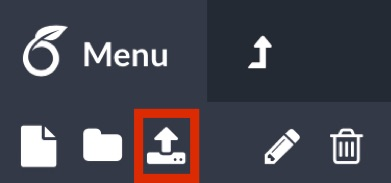
\includegraphics[width=4cm]{fig_upload.jpg}
\end{center}

\item 図を入れるには,プリアンブルに

\begin{minted}[fontsize=\small,frame=single]{latex}
\usepackage{graphicx}
\end{minted}

を付け加え,図を入れたい箇所に

\begin{minted}[fontsize=\small,frame=single]{latex}
\begin{figure}[htbp]
    \includegraphics[width=幅]{ファイル名}
\end{figure}
\end{minted}
を挿入する
\end{itemize}
\end{frame}

%%%%%%%%%%%%%%%%%%%%%%%%%%%%%%%%%%%%%%%%%%%%%%%%%%%%%%%%%%%%%%%%%%%%%%%%%%%%%%%
%%%%%%%%%%%%%%%%%%%%%%%%%%%%%%%%%%%%%%%%%%%%%%%%%%%%%%%%%%%%%%%%%%%%%%%%%%%%%%%
%%%%%%%%%%%%%%%%%%%%%%%%%%%%%%%%%%%%%%%%%%%%%%%%%%%%%%%%%%%%%%%%%%%%%%%%%%%%%%%
\begin{frame}[fragile]{文献の引用}
\begin{itemize}
\item 文献リストを出力したいところ(文末など)に次のように書く:
\begin{minted}[fontsize=\small,frame=single]{latex}
\begin{thebibliography}{99}
  \bibitem{文献1} 著者、文献名、出版社、発行年など
  \bibitem{...}  ...
\end{thebibliography}
\end{minted}
\item \cmdbs{bibitem} には文献名を表す分かりやすい名前をつけておく

\bigskip
\item 本文で文献を引用したいところで次のように書く:
\begin{minted}[fontsize=\small,frame=single]{latex}
この定理の証明は \cite{文献1} を参照されたい
\end{minted}
\end{itemize}
\end{frame}

%%%%%%%%%%%%%%%%%%%%%%%%%%%%%%%%%%%%%%%%%%%%%%%%%%%%%%%%%%%%%%%%%%%%%%%%%%%%%%%
%%%%%%%%%%%%%%%%%%%%%%%%%%%%%%%%%%%%%%%%%%%%%%%%%%%%%%%%%%%%%%%%%%%%%%%%%%%%%%%
%%%%%%%%%%%%%%%%%%%%%%%%%%%%%%%%%%%%%%%%%%%%%%%%%%%%%%%%%%%%%%%%%%%%%%%%%%%%%%%
\begin{frame}[fragile]{レポート作成の例}
\begin{itemize}
\item \bftt{jsarticle} クラスを使って日本語レポートを作成する

\begin{minted}[fontsize=\small,frame=single]{latex}
\documentclass[uplatex,dvipdfmx]{jsarticle}

\usepackage{amsmath,amssymb}
\usepackage{bm}  %太字を出すパッケージ

\title{タイトル} %\LaTeX 講習会レポート
\author{名前}    %名前+学籍番号
\date{日付}      %2022年9月29日

\begin{document}
\maketitle       %タイトルを表示

本文
\begin{thebibliography}{99} %参考文献
    \bibitem{文献1} ...
\end{thebibliography}
\end{document}
\end{minted}

\end{itemize}
\end{frame}

%%%%%%%%%%%%%%%%%%%%%%%%%%%%%%%%%%%%%%%%%%%%%%%%%%%%%%%%%%%%%%%%%%%%%%%%%%%%%%%
%%%%%%%%%%%%%%%%%%%%%%%%%%%%%%%%%%%%%%%%%%%%%%%%%%%%%%%%%%%%%%%%%%%%%%%%%%%%%%%
%%%%%%%%%%%%%%%%%%%%%%%%%%%%%%%%%%%%%%%%%%%%%%%%%%%%%%%%%%%%%%%%%%%%%%%%%%%%%%%
\begin{frame}{エラー処理}
\begin{itemize}
    \item どういうエラーが出たかは「Recompile」の横のボタンを押すと確認できる
    \begin{figure}
        \centering
        
\includegraphics[height=2cm]{fig_error.pdf}
    \end{figure}
    \item よくあるエラー:
    \begin{itemize}
        \item 「latexmkrc」と「main.tex」が同じフォルダ内に置かれていない
        
        \medskip
        \item コマンドのスペルミス $\Rightarrow$ Overleaf のコマンド補完機能を使う
        
        \medskip
        \item パッケージが読み込まれていない
    \end{itemize}
\end{itemize}
\end{frame}

%%%%%%%%%%%%%%%%%%%%%%%%%%%%%%%%%%%%%%%%%%%%%%%%%%%%%%%%%%%%%%%%%%%%%%%%%%%%%%%
%%%%%%%%%%%%%%%%%%%%%%%%%%%%%%%%%%%%%%%%%%%%%%%%%%%%%%%%%%%%%%%%%%%%%%%%%%%%%%%
%%%%%%%%%%%%%%%%%%%%%%%%%%%%%%%%%%%%%%%%%%%%%%%%%%%%%%%%%%%%%%%%%%%%%%%%%%%%%%%
\begin{frame}{参考文献}
\begin{itemize}
    \item 計算機実験ハンドブック:\\
    \url{https://github.com/utphys-comp/handbook/releases}
    \item Learn \LaTeX{} in 30 minutes:\\
    \url{https://www.overleaf.com/learn/latex/Learn_LaTeX_in_30_minutes}
    \item Free online introduction to \LaTeX (part 1): \url{https://www.overleaf.com/learn/latex/Free_online_introduction_to_LaTeX_(part_1)}
    \item \TeX{} Wiki(日本語 \TeX の情報):\\
    \url{https://texwiki.texjp.org}
\end{itemize}
\end{frame}

\end{document}
